\section{introduction}\label{Sec: intro}
%why data citation
%characteristics of data citation

The amount of information available online in structured datasets is rapidly increasing, and there is growing interest within both the digital library and computer science communities to be able to cite information extracted by queries over these datasets. Citations play a significant role in giving credit to those responsible for the data, and enable the data to be later found or reproduced. Much like a citation to traditional scholarly products such as journal or conference papers, a citation to the result of a query over a structured dataset should include snippets of information describing the dataset (analogous to a title), who is responsible for the dataset (e.g. the PI or contributors/curators of the data), as well as information about how to find the dataset (e.g. the http address, database version, and query). 

Several computational challenges must be addressed in developing a data citation system~\cite{BunemanEtAl2016}.  First, since the number of possible queries over a database is very large, it is infeasible to associate a citation to each query.  Instead, one should be able to specify citations for a small number of frequent queries and use them to automatically derive citations to other ``general'' queries.  Second, this  must be done with an acceptable time overhead, e.g. without adding significantly to the query response time.  Third, it is useful to allow the user to select a subset of the query result for which a citation should be generated, which we call  ``fine-grained'' citations.  This need  arises in many different scientific applications, in particular neuro-imaging \cite{HonorEtAl2016}. 


%our prior work

In prior work, we proposed a general framework to {\em automatically generate fine-grained citations for general queries} \cite{alawini2017automating,wu2018data}.
The approach is based on a model of {\em citation views}~\cite{BunemanEtAl2016,davidson2017model,DBLP:conf/pods/DavidsonBDMS17}: Frequent queries  are defined as views with associated citations. A query against the database is rewritten in terms of these views, and the associated citations used to construct a citation for \textit{each tuple in the query result}. Since a query may be rewritten by \textit{jointly} using more than one view, or there may be several \textit{alternate} ways to rewrite a query, the database owner may specify how citations are jointly or alternatively combined through \textit{policies} (see Figure~\ref{fig:DataCitationFW} for an overview).  The framework also allows for fine-grained citations: the citations for each tuple in the query result are then \textit{combined} to create a final citation for the specified subset of the result, which is given as another policy.  Policies give an interpretation for the joint, alternate and combined use operators, for example, taking the union, intersection or join of the citations.  In the remainder of the paper, we will call the model used in~\cite{wu2018data} the {\em {\rbafull} (\rba)} since it  extends query rewriting using views algorithms to work at the tuple level.

%why aggregate queries
A shortcoming of {\rba}, however, is that it addresses a limited class of queries -- (non-recursive) conjunctive queries and conjunctive views -- and cannot be used in applications in which the queries and views involve aggregate (such as SUM, MIN, AVG) or user-defined functions.  However, there is a growing number of biomedical applications which extract \textit{summaries} from data\-bases by issuing aggregate queries, in which views possibly involve aggregation. So the techniques of \cite{wu2018data} cannot be used.


One such example is Hetionet, a database that ``encodes'' biology by integrating various types of biological information from different publicly available resources~\cite{himmelstein2017systematic}.
As data is copied from these source datasets, citation information (generally in the form of traditional publication IDs) is also copied and should be propagated to the results of queries.
The majority of queries against this database involve aggregation to retrieve statistical information.
\eat{However, the majority of queries involve aggregation over the integrated dataset so the techniques of \cite{wu2018data} cannot be used.}

%why aggregate views
Another example, which requires both aggregate queries and aggregate views, is GENCODE~\cite{harrow2012gencode}, an encyclopedia of genes and gene variants whose goal is to identify all functional elements in the human genome using annotations. The gene annotation process involves a combination of automatic annotation, manual annotation, and experimental validation. For genes that are manually annotated, information is maintained about the responsible research groups. Statistics are also provided for every gene -- an {\em aggregate view} over the genes -- which has another type of citation giving credit to the creators of the aggregate view.
Common queries over GENCODE also involve aggregation. For instance, one query computes statistics for every \textit{type} of gene.

%why query rewriting using views is not enough since we need fine-grained reasoning
In this paper, we address the problem of automatically generating fine-grained citations when both the queries and views may involve aggregates.    Although at first glance it would appear that rewriting techniques for aggregate queries \cite{zaharioudakis2000answering, srivastava1996answering, galindo2001orthogonal,cohen2006rewriting,cohen2006user} could be used, these techniques reason at the schema level for the \textit{entire query result} rather than at the level of individual tuples, which is required for fine-grained citations.  
Extending the implementation in \cite{wu2018data} to use ideas from query rewriting for aggregate queries is possible when views are conjunctive views but still problematic when views involve aggregation since aggregation blurs the connection between tuples in the input relations and tuples in the result.  

Instead, to support aggregation, we use the observation pointed out in~\cite{BunemanEtAl2016,alawini2018data} that there is a strong connection between data provenance and data citation -- and the provenance of aggregate queries is well understood.
We therefore adopt a \textit{\pbafull\ (\pba)} that captures the connections between a result tuple and tuple(s) in views.
We illustrate how provenance helps in the example below.

\textbf{Example.} (See Figure~\ref{fig:DataCitationFW})  Recall that GENCODE is an encyclopedia of information about genes and gene variants.  Suppose that one of the views defined by the DBA  is $V_{gene}$, which counts the number of genes for each gene type, but only retains the gene types (groups) with more than 10 genes.  This corresponds to an aggregate query with a HA\-VING-clause in SQL.  $V_{gene}$ has an associated citation query which pulls snippets of information from the database and is formatted by the citation function as 
{\tt \{Group: `Jones Group', Source: `HAVANA Project', ...\}}.

% \begin{tabbing}
% $\lambda G.$\=$V(G, Ty, count(T)) $\hspace{1em}$:-$\=$ Transcript(T, N, Ty', G'), $\\
% \>$Gene(G, N, Ty), G = G', count(T) > 10$
% \end{tabbing}

% This view computes the total number of transcripts for each gene and only the genes with more than 10 transcripts will be retained. 
% Note that if we convert this view query into a SQL query, a having clauses will appear. 
% \begin{tabbing}
% $Q(G, Ty, count(T)) $\hspace{1em}\=$:-$\=$ Transcript(T, N, Ty', G'), $\\
% \>$Gene(G, N, Ty), G = G', Ty = `TEC$'
% \end{tabbing}
Now suppose that a query $Q$ counts the number of genes \textit{whose gene ids are smaller than 50} for every gene type. Then some tuples in the query result will appear in $V_{gene}$, and therefore carry the associated citation.  This is true for the first result tuple in Figure~\ref{fig:DataCitationFW},  where we assume that gene type TEC only includes genes whose ids are smaller than 50 and has at least 10 such genes.  Other tuples in the query result may not appear in $V_{gene}$, i.e. gene types which include some genes with ids 50 or greater (which we assume for the second result tuple rRNA)  or which include fewer than 10 genes.  In this case, the tuple would not carry the citation associated with $V_{gene}$.

Traditional query rewriting using views techniques would conclude that $V_{gene}$ is {\em not useful} for $Q$.  Furthermore, the \rba\ tuple-level techniques proposed in~\cite{wu2018data} could not detect whether $V_{gene}$ is useful for a given tuple in the result of $Q$.
However reasoning over the {\em provenance} of result  and view tuples could detect that TEC exists in the view instance (by comparing provenance polynomials) and that all tuples in the group have ids smaller than 50 (by finding the gene ids associated with the provenance tokens).  Thus, if the user in Figure~\ref{fig:DataCitationFW} selects TEC as the subset of interest in the query result, the citation for $V_{gene}$ ({\tt \{Group: "Jones Group", Source: "HAVANA Project", ...\}}) would be returned.

% whether current view instance $V(D)$ retains enough tuples to compute $t_q$ can be determined by {\em provenance}. If there exists one view tuple $t_v$ sharing the same provenance with $t_q$, then it implies that both $t_q$ and $t_v$ originate from the same set of base relation tuples and thus the citations of $t_q$ can be constructed by the citations of $t_v$.
%apply provenance
% Some researchers from digital library domain attempt to enable {\em provenance} property in data citation. For example, Dataverse proposes the use of provenance in data citation in their latest project ``Citation++''\footnote{https://dataverse.org/presentations/citation-data-citation-provenance-and-documentation}. However, Dataverse only generate citations for the entire dataset without providing finer-grained citations. Moreover, it cannot handle automatic citation generation for general queries. 

\textbf{Approach.} Using provenance, we develop a citation system called ProvCite, whose architecture is shown in Figure \ref{fig:DataCitationFW}; the key differences between ProvCite and the \rba\ implementation in~\cite{wu2018data} are indicated by red stars. The system executes over a provenance-enabled relational database system; here we are using GProM~\cite{arab2018gprom}.
As in \cite{wu2018data}, the DBA defines the citation views and policies to be used.  When a query is submitted, all potential {\em view mappings} are computed, which represent how views can potentially rewrite this query.  The decision of which views are valid, however, depends on the particular result tuple (as illustrated above), and for this the provenance of the result tuple is compared with the provenance of view tuples. While the user is presented with the query result and examines it to determine the subset of interest, \textit{covering sets} are calculated from the valid views for every result tuple, representing alternate rewritings in which sets of views are jointly used. So when the result subset is selected, the citation for the selected query subset can be immediately generated.   

Our initial fear in developing ProvCite was that, although the approach is interesting since it develops a novel connection between citation and provenance, it would be unacceptably slow.
To be practical, the citation should be generated without significantly extending the query time.
%and (as will be seen in the  (e.g. less than 10 seconds).  
However, since in the worst case the number of possible covering sets may be exponential in the mapping between the views and the query, the number and size of the views can be large, the number of result tuples can be large, and provenance expressions are big, this would seem to be an impossible task.  \textit{Surprisingly, the results of this paper not only show that \pba\ is feasible and extends results in \cite{wu2018data} to aggregate queries and views, but that our optimized computation allows it to even outperform our previous \rba\ approach in some cases.}

\eat{In order to use provenance for citation reasoning, one {\em provenance system} called ``GProM''\cite{arab2018gprom}\footnote{We are extremely grateful to Boris Glavic for his invaluable support in instructing us to use gprom's source code} is applied to construct the provenance-enable database engine, which retrieve provenance of the query and every view to be used to reason about valid {\em view mapping}s for every query tuples.}
\eat{
Following the same ideas in \cite{wu2018data}, a set of such {\em view mappings} construct {\em covering sets}, each of which represents one single citation. Eventually, Formatted citations, such as JOSN-format citations are generated by applying {\em policies} defined by DBAs, i.e. \{Contributors: Jones Group, Gene Type: `TEC', Query\_id: 101, Source: HAVANA project\}. How {\em covering sets} are constructed from {\em view mappings} and how {formated citations} are produced have been explored in \cite{wu2018data} and will not be repeated here. Instead, how to reason about valid view mappings for each individual tuple level in the context of aggregate queries and  aggregate views becomes our major concerns in this paper.}

\begin{figure}[t!]
    \centering
    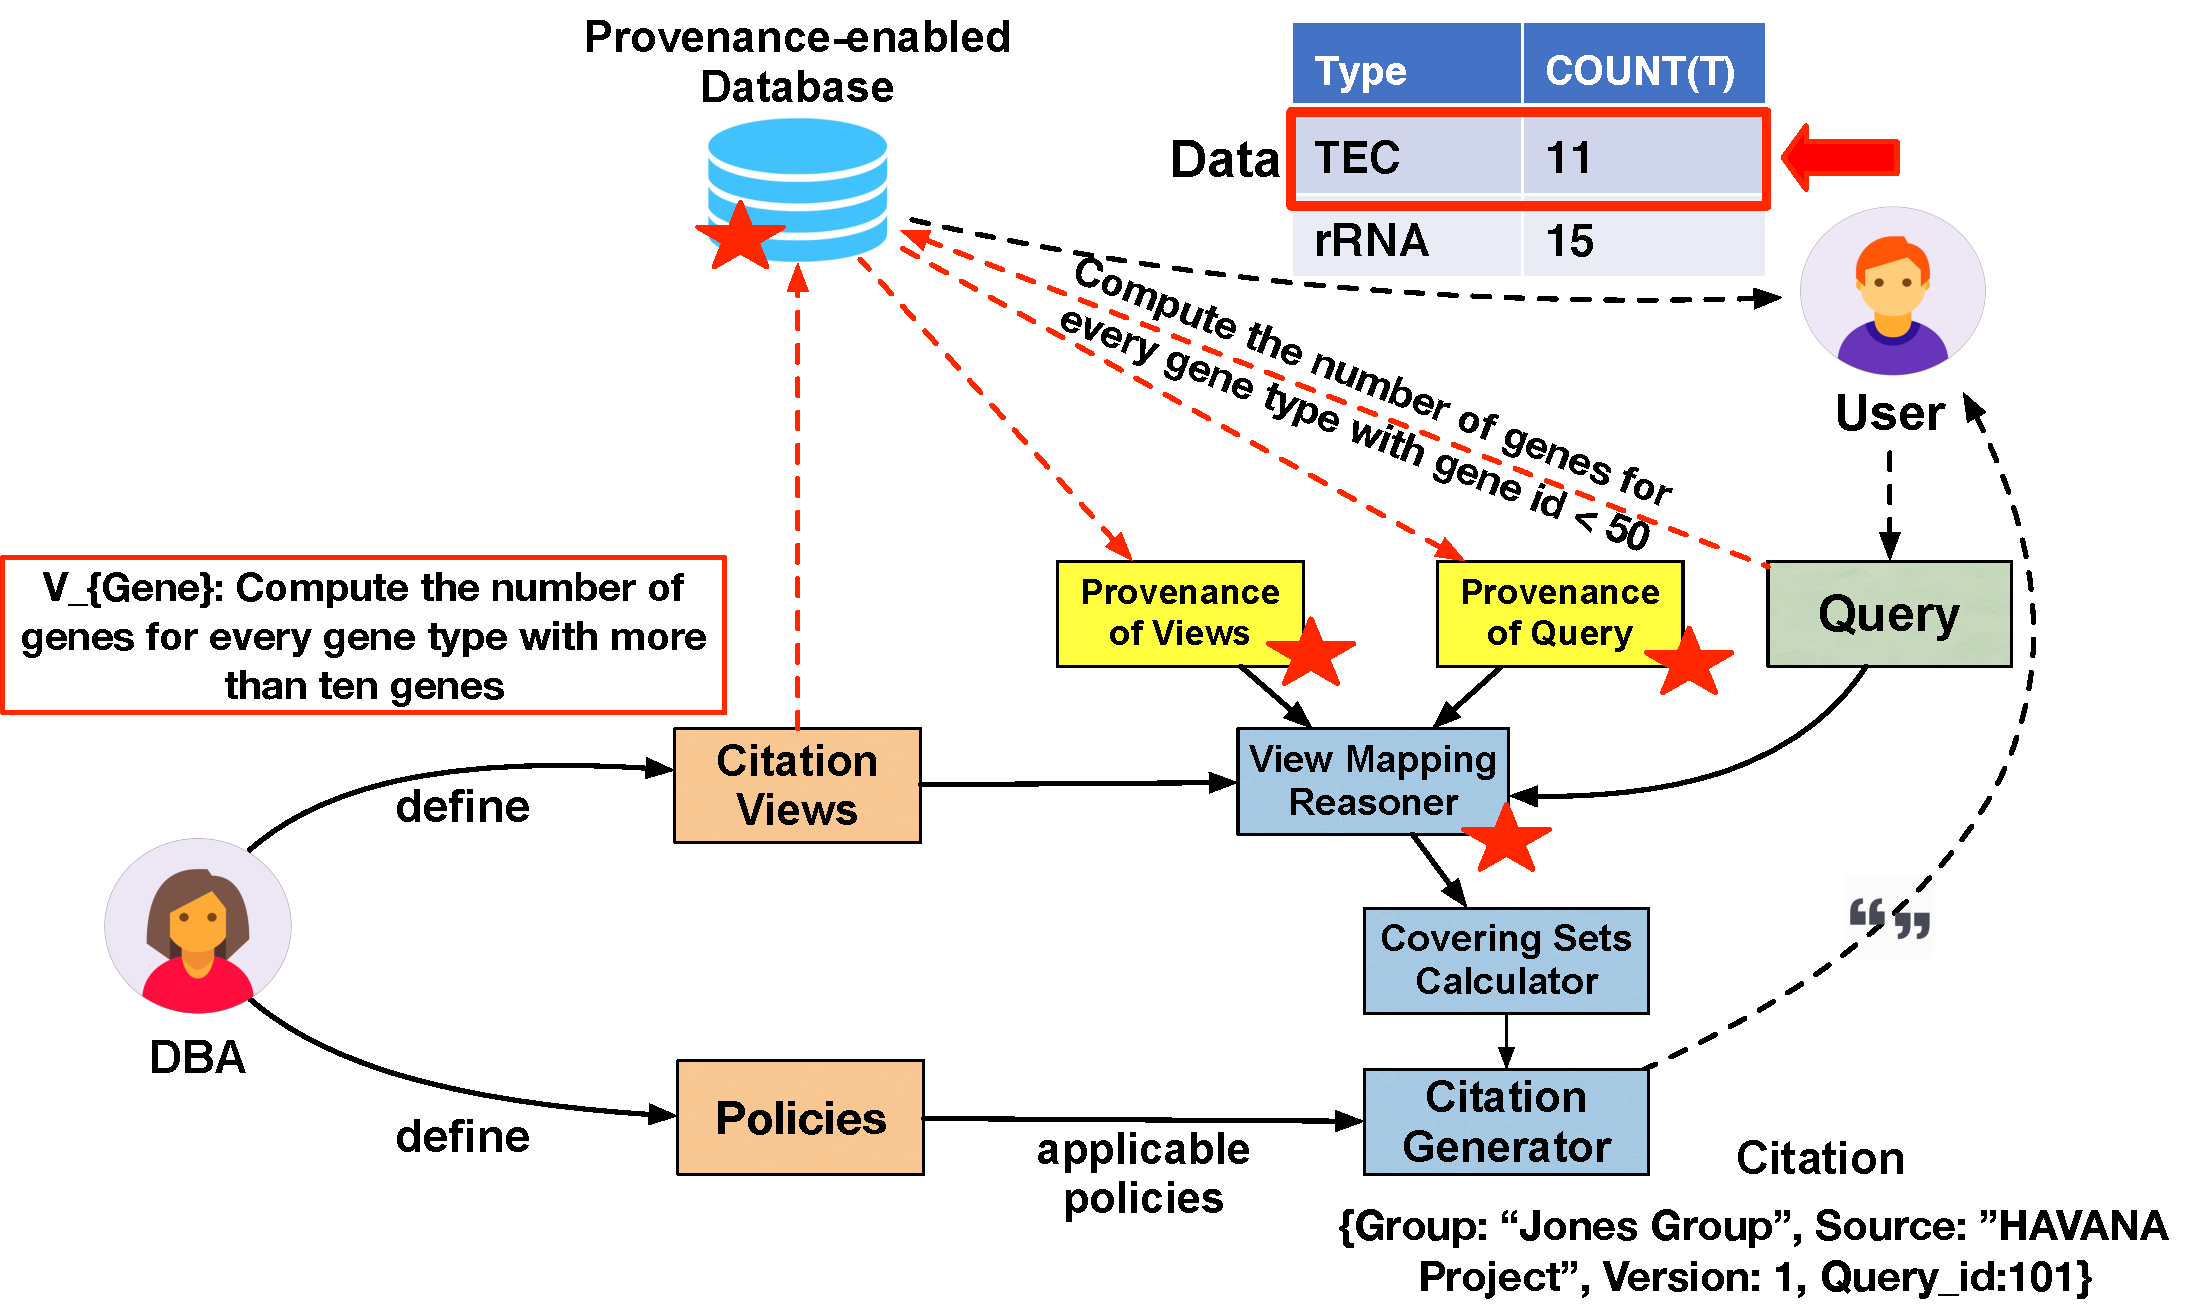
\includegraphics[width=0.48\textwidth,height=0.25\textwidth]{Figures/general_citaiton_framework.pdf}
    \caption{System overview of ProvCite}
    \small \label{fig:DataCitationFW}
\end{figure}

%contributions
{\textbf{Contributions}} of this paper include:
\begin{enumerate}
\item A framework formalizing the connection between data provenance and data citation.
\item %\scream{claim general agg function is supported} 
A semantics for generating citations to the results of aggregate queries with {\em general aggregate functions} given a set of either aggregate or conjunctive views using provenance in the view and query instances. 
\item An implementation of the \pba\ called ProvCite, which automatically generates fine-grained citations for the results of general queries, where both the queries and views may involve aggregates. Some optimization strategies were used, which are also applicable in other scenarios wherever the provenance from different queries or views needs to be compared, such as fine-grained access control \cite{goyal2006attribute} and linked brushing in data visualization \cite{psallidas2018smoke}.

\eat{Two strategies are tested for the provenance of views: In the first, provenance is generated on the fly ({\em lazy strategy}), whereas in the second provenance is pre-computed ({\em eager strategy}).}
\item 
Experiments using both {\em synthetic}  and {\em realistic} workloads, comparing 
\provalg\ against \rba\ approaches~\cite{wu2018data} in the case of aggregate queries and conjunctive views, and measuring the effect of the optimization strategies for \provalg\ when queries and views involve aggregates.  
\eat{ In {\em synthetic workloads}, the new approach is compared to prior approaches (TLA and SSLA) in the case where all views are $\mathcal{CV}$ while ({\em virtualization strategy}) and ({\em materialization strategy}) are compared to each other in the case where all views are $\mathcal{CAV}$ (which cannot be handled by TLA or SSLA).}
The results show that \provalg\ has acceptable time performance even when the queries and views have large instances, and can in some cases significantly outperform \rba\ approaches.
\eat{feasible in time performance no matter whether the provenance of views are materialized or virtual even when queries and views have large instances; 2) compared to TLA and SSLA, the provenance approach is even about 2x faster than TLA and SSLA in some cases. }
\end{enumerate}

\eat{Yinjun, there are too many sections.  Perhaps fold background information into the model, and/or the algorithm?}
The rest of this paper is organized as follows.
Related work is discussed in Section~\ref{Sec: related_work}, and the running example and preliminaries are given in Section~\ref{Sec: examples}.  Details of the \pba\ and its implementation in ProvCite are presented in Sections~\ref{sec: model} and~\ref{Sec: implementation} respectively. Section~\ref{sec:experiments} gives experimental results before concluding in Section~\ref{sec: conclusion}.


% We have developed a model for automating data citation and implemented three approaches for generating citations at various levels of granularity (tuple level, semi-schema level, and schema level)~\cite{wu2018data}.  The model, however, only works for non-recursive conjunctive queries ($\mathcal{CQ}$) and non-recursive conjunctive views ($\mathcal{CV}$). In this work, we propose a model that uses {\em provenance} to support more complicated queries, i.e. non-recursive select-project-join-aggregate (SPJA) queries ($\mathcal{CAQ}$) and non-recursive select-project-join-aggregate (SPJA) views ($\mathcal{CAV}$). In both $\mathcal{CAQ}$ and $\mathcal{CAV}$, the aggregate operator can only occur as the last step in the query plan (no aggregation in sub-queries), and may have conditions over aggregates (i.e, the HAVING clause)

% In this section, we assume that the form of both the query and views is . 
% To represent such  queries, we use an extended version of Datalog called S-Datalog \cite{consens1990low}, an extension which is commonly used in work on query rewriting using views with aggregation \cite{cohen2006user}\cite{cohen2006rewriting}. In this section, the aggregate operator can only occur as the last step in the query plan (no nesting), and may have conditions over aggregates (i.e, the HAVING clause in SQL) in views and queries, which is not considered in \cite{cohen2006rewriting}.


% \subsection{Why aggregate queries and views}
% In several applications, we have found that users are interested in extracting \textit{summaries} from a database by issuing aggregate queries. 

% Although aggregate queries are common in Hetionet, the citable objects (view queries) are in $\mathcal{CV}$. In this case the reasoning is not very different from the conjunctive query case. 
% We therefore have another example, GENCODE\footnote{www.gencodegenes.org}, where \textit{both the queries and views} are $\mathcal{CAQ}$.  In this case, the reasoning becomes more interesting.

% Since neither of these examples are intuitive, in the paper (to be written) we will develop complex queries and views using a database of computer science publications (extracted from DBLP) and funding sources (extracted from the NSF website).  We will mention, but not build on, the use cases of Hetionet, IUPHAR and GENCODE.
